% ==========================================
% INTRODUCTION
% ==========================================

\newpage
\pagenumbering{arabic}

\chapter{GIỚI THIỆU}

\begin{concept}[15cm]
\textit{Nội dung chương này sẽ tập trung giới thiệu tổng quan về đề tài, cụ thể về hệ thống BE-PUM và cách thức xây dựng mô hình của BE-PUM, đồng thời giới thiệu về packer, phương pháp model checking và và công cụ NuSMV; mục tiêu cụ thể hướng tới của đề tài và phạm vi thực hiện của đề tài, những kết quả ban đầu đã đạt được của quá trình nghiên cứu đề tài, cũng như cấu trúc của luận văn cũng sẽ được giới thiệu cụ thể.}
\end{concept}

\section{Tổng quan đề tài}

\subsection{Tổng quan về hệ thống BE-PUM}

\hspace{0.5cm}Binary Emulation for PUshdown Model (BE-PUM) là công cụ với lõi được xây dựng dựa trên framework Jackstab - một thư viện mã nguồn mở được xây dựng cho phép dịch ngược mã nhị phân, nói cách khác Jackstab hỗ trợ chuyển đổi từ những giá trị mã máy thành hợp ngữ cấp cao, ngoài ra Jackstab cũng cho phép phân tích tĩnh một tập tin thực thi. Dựa trên cơ sở đó, BE-PUM được xây dựng với mục tiêu xây dựng một mô hình thực thi hoàn chỉnh của một tập tin mã nhị phân nói chung và cụ thể hơn là malware, cũng như những tập tin được đóng gói bởi các công cụ packer, mô hình đó được biểu diễn thông qua Control Flow Graph (CFG) của chương trình.\\ 

\hspace{0.5cm}CFG được sinh ra bởi hệ thống BE-PUM biểu diễn mô hình của tập tin được phân tích, hay nói cách khác biểu diễn luồng điều khiển của chương trình. Trong hệ thống BE-PUM, một node của CFG tương ứng với một node trong CFG, và một edge trong mô hình của BE-PUM được biểu diễn là cạnh nối giữa 2 node trong CFG. Quá trình sinh mô hình được thực hiện thông qua giải thuật On-the-fly model generation. Hình \ref {fig:IntroCFG} mô tả CFG sau khi tập tin với đoạn mã \ref {lst:IntroASM} được phân tích trong hệ thống BE-PUM.

\begin{code}
\begin{lstlisting}[captionpos=b,caption={Đoạn mã thực thi Assembly},label={lst:IntroASM},frame=single]
00401000	inc eax
00401001	jne 0x00401000
00401006 	push eax		
\end{lstlisting}
\end{code}

\begin{figure}
\centering
\begin{tikzpicture}[shorten >=1pt,node distance=2cm,on grid,auto] 
   	\node[cfgstate,align=center](s_1){0x00401000\\\ inc \%eax}; 
   	\node[cfgstate,align=center](s_2)[below of=s_1]{0x00401001\\\ jne 0x00401000};
   	\node[cfgstate,align=center](s_3)[below of=s_2]{0x00401006\\\ pushl \%eax};
    \path[-{>[scale=2,length=3,width=3]}] 
    (s_1) edge node {} (s_2)
  	(s_2.east) edge [bend right=60] node {} (s_1.east)
    (s_2) edge node {} (s_3);	  
\end{tikzpicture}
\caption{CFG của BE-PUM với đoạn mã assembly \ref {lst:IntroASM}}
\label{fig:IntroCFG}
\end{figure}

\hspace{0.5cm}Kế thừa bộ thư viện dịch ngược mã nhị phân của Jackstab, với mục tiêu có thể xây dựng hoàn chỉnh mô hình cho các tập tin thực thi, BE-PUM không chỉ dừng lại với việc phân tích tĩnh mà còn mở rộng để có thể phân tích động thông qua việc áp dụng các kỹ thuật bao gồm:

\begin{itemize}
\item{Dynamic symbolic execution: kỹ thuật nhằm tính toán các giá trị thanh ghi và bộ nhớ cụ thể từ đó có thể giải quyết vấn đề xử lý kỹ thuật trong đó sử dụng các câu lệnh nhảy động, nhảy có điều kiện - một kỹ thuật được sử dụng rất phổ biến trong hầu hết các malware và packer.\\}
\item{On-the-fly model generation: giải thuật chính được áp dụng trong hệ thống BE-PUM, do quá trình thực thi của tập tin mã nhị phân là thực thi động, do đó quá trình này sẽ bao gồm một dãy các câu lệnh mã nhị phân liên tiếp bắt đầu từ một giá trị trong bộ nhớ ở phân vùng mã, giá trị địa chỉ này được trỏ tới bởi giá trị thanh ghi EIP. Chính việc áp dụng giải thuật On-the-fly mà vấn đề thay đổi động giá trị opcode của các câu lệnh trong quá trình thực thi được giải quyết một cách triệt để, hay nói cách khác với những tập tin thực thi có sử dụng kỹ thuật self-modifcation code sẽ được BE-PUM hỗ trợ hoàn toàn.\\}
\item{Xử lý kỹ thuật obfuscation: điểm mạnh và là ưu thế vượt trội của BE-PUM so với các công cụ phân tích mã thực thi khác như Jackstab, IDA-Pro, Capstone, Unicorn, METASM, HOOPER đó là BE-PUM có hỗ trợ xử lý những kỹ thuật obfuscation như: indirect jump, self-modification code, entry point obscuring, strutured exception handling, overlapping instruction những kỹ thuật vốn được sử dụng rất phổ biến trong malware hay packer.}
\end{itemize}

\begin{code}
\begin{lstlisting}[captionpos=b,caption={Đoạn mã thực thi dưới dạng ASM},label={lst:ASMReal},frame=single]
start:
	cmp eax, 0
	jne A2
A1:
	add eax, 09h
	inc eax
	inc eax
	jmp eax
A2:
	mov eax, ss:[esp]
	ret
A3:
	push 0
	call ExitProcess
end start
\end{lstlisting}
\end{code} 

\begin{figure}
\centering
\begin{tabular}[c]{cc}
	\subfloat[BE-PUM]
	{
		\label{fig:BEPUMReal}
		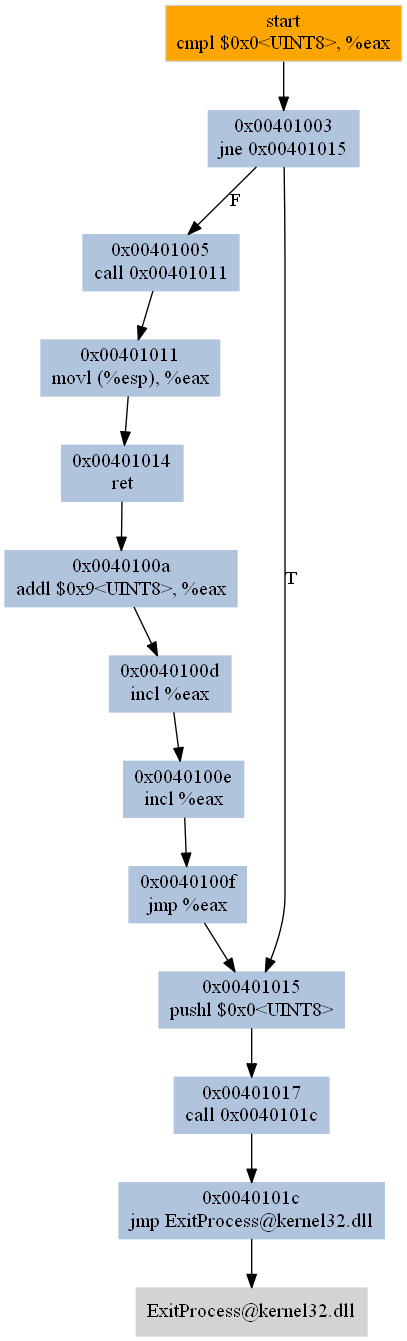
\includegraphics[width=0.4\textwidth]{bepum_sample}
    }
    &
	\subfloat[IDA-Pro]
	{
		\label{fig:IDAReal}
        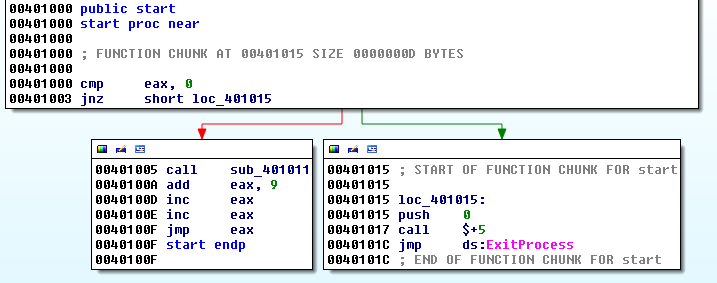
\includegraphics[width=0.6\textwidth]{ida_sample}
	}
\end{tabular}
\caption{Mô hình của BE-PUM và IDA Pro được sinh ra từ đoạn mã \ref {lst:ASMReal}}
\label{fig:ModelReal}
\end{figure}

\hspace{0.5cm}Hình \ref {fig:ModelReal} cho thấy công cụ IDA Pro, một công cụ rất mạnh được sử dụng cho quá trình phân tích tập tin mã nhị phân không thể xử lý kỹ thuật Indirect Jump tại câu lệnh JMP EAX tại vị trí 0x0040100f, cụ thể IDA Pro sẽ dừng thực thi và không nhảy đến được vị trí 0x00401015. Ngược lại hệ thống BE-PUM xử lý và nhảy đến vị trí 0x00401015 đã được tính toán trước đó.

\subsection{Tổng quan về Packer}

\begin{figure}
\centering
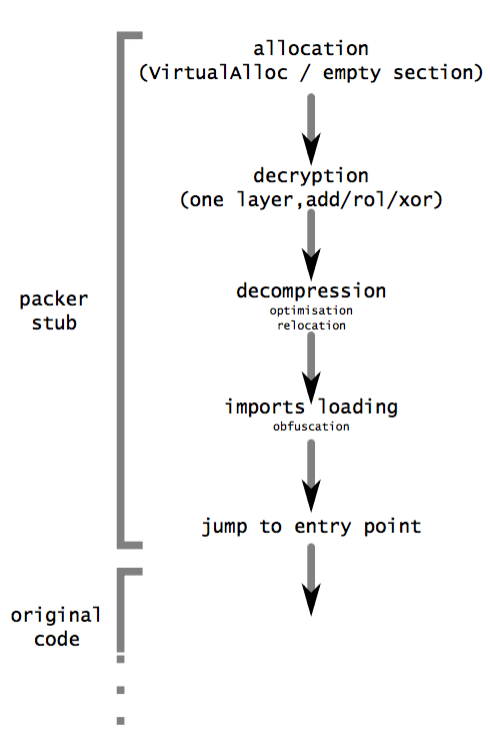
\includegraphics[width=0.5\textwidth]{simple_packer_schema}
\caption{Mô hình của một packer đơn giản}
\label{fig:PackerSchema}
\end{figure}

\hspace{0.5cm}Packer là những công cụ dùng để đóng gói một tập tin. Hình \ref {fig:PackerSchema} mô tả cấu trúc của một packer đơn giản. Trong đó có thể thấy mục tiêu chính của một packer có thể được chia làm 3 mục tiêu cụ thể là:

\begin{itemize}
\item{Giảm kích thước của tập tin: đây cũng là mục tiêu mà rất nhiều packer hướng tới, bằng việc áp dụng các kỹ thuật packing và self-unpacking, encryption và self-decryption, mà kích thước của một tập tin được đóng gói qua đó cũng giảm đi một cách đáng kể. Tuy nhiên, những packer hiện đại ngày nay đã không còn đặt tiêu chí giảm kích thước tập tin lên hàng đầu, bởi giảm kích thước đồng nghĩa với việc sử dụng những kỹ thuật bảo mật khác sẽ được loại bỏ và do đó độ tin cậy của một packer cũng giảm đi. Thậm chí những packer có cơ chế bảo mật tốt hiện nay có thể kể ra như Armadillo, Themida hay PEBundle có thể làm kích thước tập tin tăng lên rất nhiều lần do việc áp dụng kỹ thuật phức tạp của những packer này trên tập tin cần đóng gói là rất nhiều.\\}
\item{Chống dịch ngược: một trong những kỹ thuật được sử dụng rất nhiều trong việc tìm ra những lỗ hỏng của một phần mềm từ đó tìm cách đánh cắp dữ liệu mật của phần mềm đó hay tìm hiểu cơ chế sinh khoá, dịch ngược cũng được áp dụng để phát hiện những kỹ thuật malware từ đó tìm cách sửa lỗi hệ thống mà malware khai thác và chống lại malware đó. Nhằm chống lại kỹ thuật dịch ngược, packer cũng được sử dụng như một công cụ hiệu quả vì những giải thuật đóng gói tập tin phức tạp của packer có thể khiến việc dịch ngược mã nhị phân trở nên vô cùng khó khăn.\\}
\item{Bảo vệ bản quyền của phần mềm: đây cũng là mục tiêu chính yếu nhất mà các packer ngày nay hướng tới, bằng cách nâng cao độ phức tạp của các giải thuật đóng gói, đồng thời áp dụng những kỹ thuật anti-debugging, anti-reversing sẽ qua đó giúp bảo vệ một phần mềm khỏi việc đánh cắp thông tin bất hợp pháp. Malware cũng lợi dụng điểm mạnh này của packer nhằm che dấu quá trình thực thi của mình.}
\end{itemize}

\subsection{Tổng quan về Model Checking}

\hspace{0.5cm}Bài toán kiểm định các hệ thống phần mềm hay phần cứng là một bài toán vô cùng quan trọng và tốn rất nhiều thời gian và công sức nếu được thực hiện một cách thủ công, do đó việc đề ra một phương thức tự động nhằm kiểm định hệ thống là yêu cầu cần thiết được đề ra nhằm giải quyết vấn đề này. Chính vì điều này, mà việc xây dựng một phương pháp hình thức hay nói cách khác là việc áp dụng toán học để xử lý bài toán kiểm định sẽ mang lại hiệu quả và giảm rất nhiều thời gian, công sức.\\

\hspace{0.5cm}Model checking được xây dựng bởi Edmund Melson Clarke và Ernest Allen Emerson, cũng như Jean-Pierre Queille và Joseph Sifakis Jean-Pierre ra đời để giải quyết bài toán này. Model checking là một kỹ thuật kiểm định tự động một mô hình hệ thống với một đặc tả các tính năng của mô hình đó dưới dạng công thức logic có yếu tố thời gian. Bằng cách duyệt toàn bộ không gian trạng thái của mô hình đó, phương pháp model checking sẽ chứng minh mô hình có thoả mãn các tính chất đã được mô tả trước đó hay không.

\subsection{Tổng quan về NuSMV}

\hspace{0.5cm}NuSMV là một công cụ kiểm tra mô hình dạng ký hiệu mã nguồn mở, là một dự án kết hợp giữa ITC-IRST, viện nghiên cứu ở phía Đông Trento, Ý và đại học Carnegie Mellon. Chính vì mã nguồn mở mà thông qua đó có thể dễ dàng thay đổi mã nguồn để có thể cung cấp thêm nhiều tính năng và hỗ trợ tốt hơn, nâng cao hiệu suất kiểm tra mô hình trên hệ thống có số trạng thái hữu hạn.\\

\hspace{0.5cm}Giống như những công cụ kiểm tra mô hình khác, NuSMV cũng cần đầu vào là một mô hình cần được kiểm tra và một mô tả dưới dạng công thức luận lý có yếu tố thời gian để thực hiện việc kiểm tra mô hình. Mô hình NuSMV được biểu diễn dưới dạng ngôn ngữ SMV, NuSMV hỗ trợ cả CTL model checking và LTL model checking.

\section{Mục tiêu đề tài}

\hspace{0.5cm}Hệ thống BE-PUM được phát triển để có thể xây dựng được mô hình chính xác của chương trình thực thi, cụ thể là mô hình quá trình thực thi của malware, từ đó có thể nhận dạng được malware. Tuy nhiên, việc malware sử dụng packer để ẩn thân khiến quá trình xây dựng này trở nên khó khăn. Xuất phát từ khó khăn thực tế đó, mục tiêu của đề tài luận văn tốt nghiệp này hướng tới bao gồm:

\begin{itemize}
\item{Phân tích những kỹ thuật được sử dụng của các packer bao gồm nhóm kỹ thuật obfuscation, kỹ thuật anti-reversing, anti-debugging.\\} 
\item{Hỗ trợ hệ thống BE-PUM xử lý các kỹ thuật của packer để đảm bảo BE-PUM có thể phân tích hoàn toàn các packer, cụ thể, tìm ra được vị trí entry point thực sự của tập tin được đóng gói. Từ đó, có thể xây dựng chính xác mô hình quá trình thực thi của tập tin.\\}
\item{Nhận dạng packer thông qua chữ ký bằng phương pháp nhận dạng chữ ký được sử dụng trong thực tế.\\}
\item{Nhận dạng packer thông qua ngữ nghĩa bằng phương pháp model checking, cụ thể, kết hợp hệ thống BE-PUM và công cụ kiểm tra mô hình dạng ký hiệu NuSMV để kết luận một tập tin có đang được đóng gói bởi packer nào hay không.\\}
\item{So sánh độ hiệu quả giữa hai phương pháp nhận dạng packer, một là phương pháp nhận dạng chữ ký và hai là phương pháp nhận dạng ngữ nghĩa.}
\end{itemize}

\section{Phạm vi đề tài}

\hspace{0.5cm}Với những giới hạn trong việc chuyển đổi giữa mô hình của BE-PUM và mô hình của NuSMV, cũng như những khó khăn khi phân tích những packer hiện đại mà đề tài luận văn bao gồm những hạn chế cụ thể như sau:

\begin{itemize}
\item{Dữ liệu chữ ký của packer được sử dụng từ dữ liệu mở của phần mềm CFF Explorer, do đó BE-PUM chỉ hỗ trợ nhận dạng chữ ký những packer trong giới hạn cụ thể được định nghĩa tương tự như trong CFF Explorer.\\}
\item{Do sự phức tạp trong việc sử dụng kỹ thuật mới đòi hỏi xử lý Process, Thread phức tạp của các packer hiện đại như: Armadillo, Fastpack, Themida, PEBunble, mà những kỹ thuật này chưa được hỗ trợ hoàn toàn trong BE-PUM nên hiện tại BE-PUM chưa xử lý được những packer này, giới hạn đề tài chỉ hỗ trợ 27 packer.\\}
\item{Do BE-PUM chỉ xử lý được 27 packer và 13 kỹ thuật được sử dụng trong packer, nên giới hạn đề tài chỉ hỗ trợ nhận dạng 27 packer thông qua kiểm tra mô hình dựa trên mô tả của 13 kỹ thuật này.}
\end{itemize}  

\section{Kết quả đề tài}

\hspace{0.5cm}Nội dung và kết quả nghiên cứu được thực hiện trong đề tài luận văn này đã được vinh dự đóng góp trong bài báo "Precise Packer detection using Model checking" tại hội nghị SEATUC 2016 (10th SOUTH EAST ASIAN TECHNICAL UNIVERSITY CONSORTIUM SYMPOSIUM) được diễn ra tại Viện công nghệ Shibaura, Tokyo, Nhật Bản từ ngày 22/02/2016 đến ngày 24/02/2016.

\section{Cấu trúc của luận văn}

\hspace{0.5cm}Nội dung của luận văn tốt nghiệp bao gồm các chương chính như sau:

\begin{itemize}
\item{\textbf{Mở đầu}: giới thiệu sơ lược về đề tài luận văn, bố cục chung của luận văn, trình bày những mục tiêu khi chọn đề tài.\\}
\item{\textbf{Chương 1}: tập trung giới thiệu tổng quan về đề tài, cụ thể về hệ thống BE-PUM và cách thức xây dựng mô hình của BE-PUM, đồng thời giới thiệu về packer, phương pháp model checking và công cụ NuSMV; mục tiêu cụ thể hướng tới của đề tài và phạm vi thực hiện của đề tài, những kết quả ban đầu đã đạt được của quá trình nghiên cứu đề tài, cũng như cấu trúc của luận văn cũng sẽ được giới thiệu cụ thể.\\}
\item{\textbf{Chương 2}: tập trung phân tích vấn đề, cụ thể là những vấn đề của hệ thống BE-PUM khi xử lý packer thông qua 3 ví dụ cụ thể về 2 packer được malware sử dụng trong thực tế, rút ra nhận xét tổng quát và những thách thức đặt ra cho đề tài. Ngoài ra, chương này cũng sẽ tập trung bàn luận về những thách thức này, từ đó đưa ra những giải pháp cụ thể để giải quyết những khó khăn đó.\\}
\item{\textbf{Chương 3}: giới thiệu những kiến thức nền và các công nghệ được sử dụng trong đề tài. Để có thể giải quyết những thách thức như chương 2 đã nêu ra, cần nắm vững kiến thức nền tảng về hệ thống BE-PUM và lý thuyết về model checking, cũng như về công cụ NuSMV. Ngoài ra chương này cũng tập trung giới thiệu cụ thể về 13 kỹ thuật được hỗ trợ trong packer.\\}
\item{\textbf{Chương 4}: trình bày về các công việc đã thực hiện trong luận văn dựa trên những kiến thức nền được giới thiệu ở chương 2. Cụ thể, chương này sẽ tập trung giới thiệu việc kết hợp giữa hệ thống BE-PUM và công cụ NuSMV trong việc nhận dạng packer. Để có thể so sánh giữa phương pháp pháp nhận dạng packer thông qua chữ ký và phương pháp model checking, giải thuật nhận dạng packer thông qua chữ ký cũng được hiện thực và giới thiệu cụ thể trong chương này.\\}
\item{\textbf{Chương 5}: chủ yếu trình bày những kết quả đã đạt được sau khi thực hiện đề tài, kết quả thí nghiệm trên tập malware thực tế, cũng như những so sánh giữa 2 phương pháp nhận dạng packer.\\}
\item{\textbf{Chương 6}: nêu ra những hạn chế được đặt ra trong quá trình thực hiện đề tài và hướng giải quyết trong tương lai để có thể khắc phục những hạn chế đó.}
\end{itemize}

